\subsubsection{Эквивалентная схема pn-перехода и совокупность ее параметров.}
Эквивалентная схема, отражающая работу полупроводникового диода имеет следующий вид:


\begin{center}
	\begin{figure}[h!]
		\center{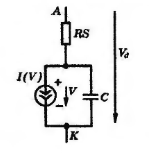
\includegraphics[scale=0.9]{pn-eqiv.png}}
		\caption{Эквивалентная схема диода}	
		\label{pic:pn-eqiv}
	\end{figure}
\end{center}

Где ток определяется из уравнения:
\begin{equation}
I = I_0 \left( e^{\frac{V}{\varphi_t}}-1 \right)
\end{equation}
Где $I_0$ - тепловой ток, значение которого является одним из параметров модели.\\
$R_s$ -объемное сопротивление, является параметром.\\
$C = C_b+ C_{dif}$ - Инерционность перехода, определяемая \\
$C_{dif} = \tau \frac{d I}{d V}$, где $\tau$ - время переноса заряда(параметр)\\
$C_b = C_{b0} \sqrt{1 - \frac{V}{\Delta \phi_0}}$, где $C_{b0}$ - барьерная емкость при нулевом смещении (параметр),
$\Delta \phi_0$ - контактная разность потенциалов (параметр)\\
\label{1_2_5}
При этом, если учитывается пробой диода, то обратный ток диода принимает следующий вид:
\begin{equation}
I_r = I_{rh} + I_{rl}
\end{equation}
\begin{equation}
I_{rh} = IBV e^{\frac{- V + BV}{\phi_t}}
\end{equation}
Где $IBV$ - начальный ток пробоя, являющийся параметром, как и $BV$- напряжение пробоя. \\

ВАХ диода в этом случае:


\begin{center}
	\begin{figure}[h!]
		\center{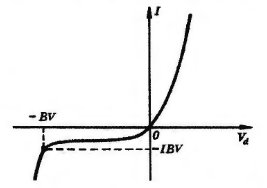
\includegraphics[scale=0.9]{pn-rev_VAH.png}}
		\caption{ВАХ при пробое у экв. схемы}	
		\label{pic:pn-rev_VAH}
	\end{figure}
\end{center}

\pagebreak
